\documentclass[manual-fr.tex]{subfiles}
\begin{document}

Une fois lancée, il faut commencer par choisir les éléments suivants :
\begin{itemize}
    \item les données qui serviront à l'entraînement;
    \item la chaîne de prétraitement pour enrichir les données.
\end{itemize}

~

Pour choisir les données qui serviront à l'entraînement, voir les figures \ref{fig:train_sem-02} et \ref{fig:train_sem-03}. Les différentes étapes sont :
\begin{enumerate}
    \item cliquer sur le bouton «~select file(s)~»;
    \item sélectionner le(s) fichiers annotés;
    \item cliquer sur «~ouvrir~».
\end{enumerate}

~

Une fois sélectionnés, les fichiers seront listés comme indiqué dans la figure \ref{fig:train_sem-03}. Il n'est pas nécessaire que les fichiers annotés soient du même format. Ces derniers peuvent avoir n'importe quel format de fichier supporté par SEM. À l'heure où cette documentation a été écrite, les fichiers supportés sont :
\begin{itemize}
    \item XML SEM, le format XML interne de SEM;
    \item json SEM, le format json interne de SEM;
    \item BRAT \cite{stenetorp2012brat};
    \item GATE \cite{cunningham2002gate};
\end{itemize}

~

Une fois les fichiers annotés choisis, il faut faire le choix de la chaîne de traitement pour prétraiter les documents. SEM propose un exemple d'une telle chaîne pour réentraîner la tâche de reconnaissance des entités nommées dans la figure \ref{fig:train_sem-02}, à savoir «~NER-train.xml~».

\begin{figure}[ht!]
    \begin{center}
    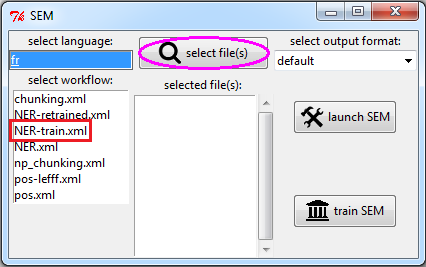
\includegraphics[scale=0.5]{fr/images/train_sem-02.png}
    \end{center}
    \caption{Entouré en violet : le bouton pour sélectionner les documents à utiliser pour l'entraînement. Encadré en rouge : la chaîne de traitement à utiliser pour entraîner un nouveau modèle.}
    \label{fig:train_sem-02}
\end{figure}

\begin{figure}[ht!]
    \begin{center}
    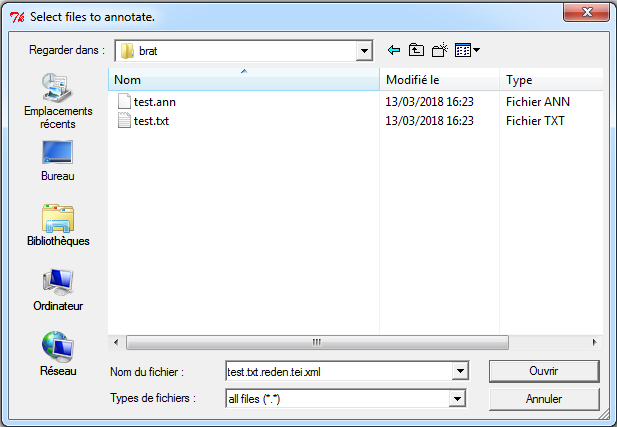
\includegraphics[scale=0.5]{fr/images/train_sem-03.png}
    \end{center}
    \caption{Des exemples de fichiers annotés au format BRAT. Ne choisir que les fichiers ".ann" ou les fichiers ".txt" pour l'entraînement.}
    \label{fig:train_sem-03}
\end{figure}

\begin{figure}[ht!]
    \begin{center}
    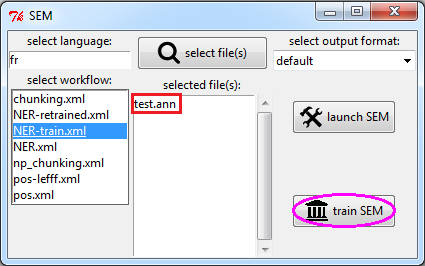
\includegraphics[scale=0.5]{fr/images/train_sem-04.png}
    \end{center}
    \caption{encadré en rouge : les documents utilisés pour l'entraînement. Entouré en violet : le bouton pour entraîner SEM.}
    \label{fig:train_sem-04}
\end{figure}

\end{document}
